\setbeamercolor{block title}{bg=blue!30,fg=black}
\setbeamercolor{block body}{bg=blue!10,fg=black}
\setbeamertemplate{blocks}[rounded][shadow=false]

\section{Introduction \& Background}
\subsection{General Introduction}
\addtocounter{framenumber}{-1}
\begin{withoutheadline}
\begin{frame}{General Introduction}{Centralized Data Centres}

\begin{block}{ The Emergence of Centralized Data Centres}
    \begin{itemize}
    \item  Number of cloud users have reached 3.4 Billions in 2018.
    \item Centralized data centres are cost effective. 
    \item The big players rely on nothing more than 15 data centres. 
    \item<2-> Two main problems: internet traffic and high latency.  
    \end{itemize}
\end{block}



\begin{figure}[p]

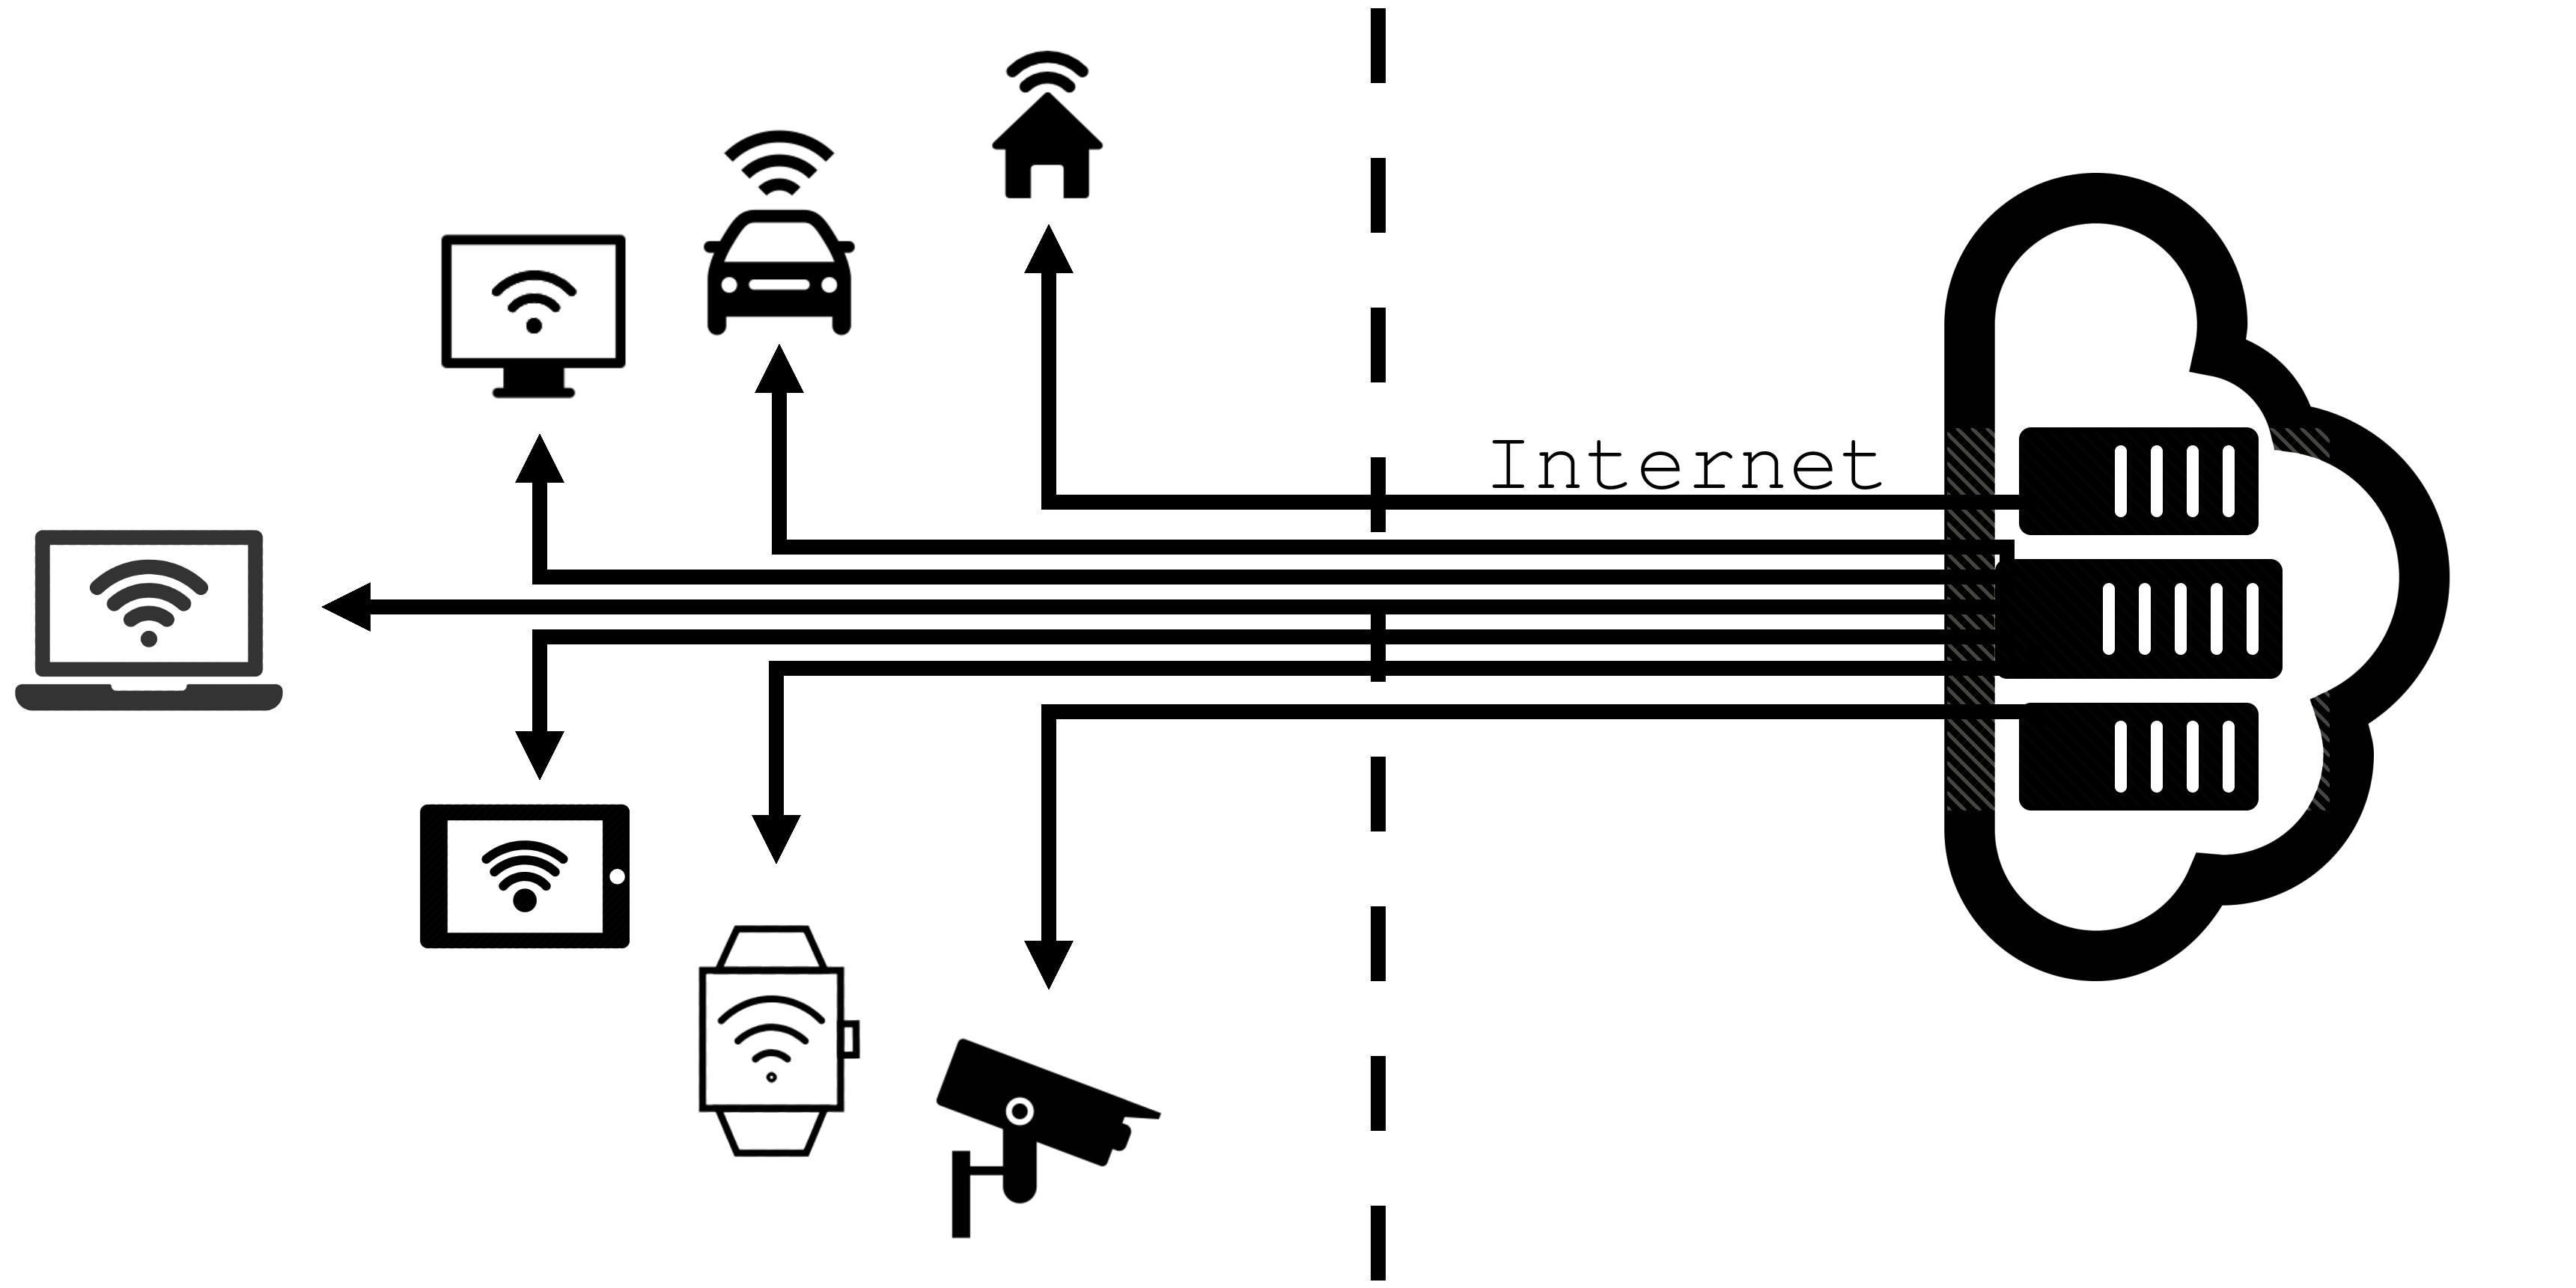
\includegraphics[width=0.8\linewidth]{figures/cloud.png}
  
\end{figure}
\end{frame}
\end{withoutheadline}


\subsection{The Fog}
%\addtocounter{framenumber}{-1}
\begin{withoutheadline}
\begin{frame}{The Fog}

\begin{block}{Greedy Applications and The Fog}
    \begin{itemize}
    \item Fog computing an extended paradigm of clouds.
    \item Nodes will be distributed in the  end-user proximity.
    \item Fog will provide lower latencies and data localization.
    \end{itemize}
\end{block} 

\begin{figure}[p]

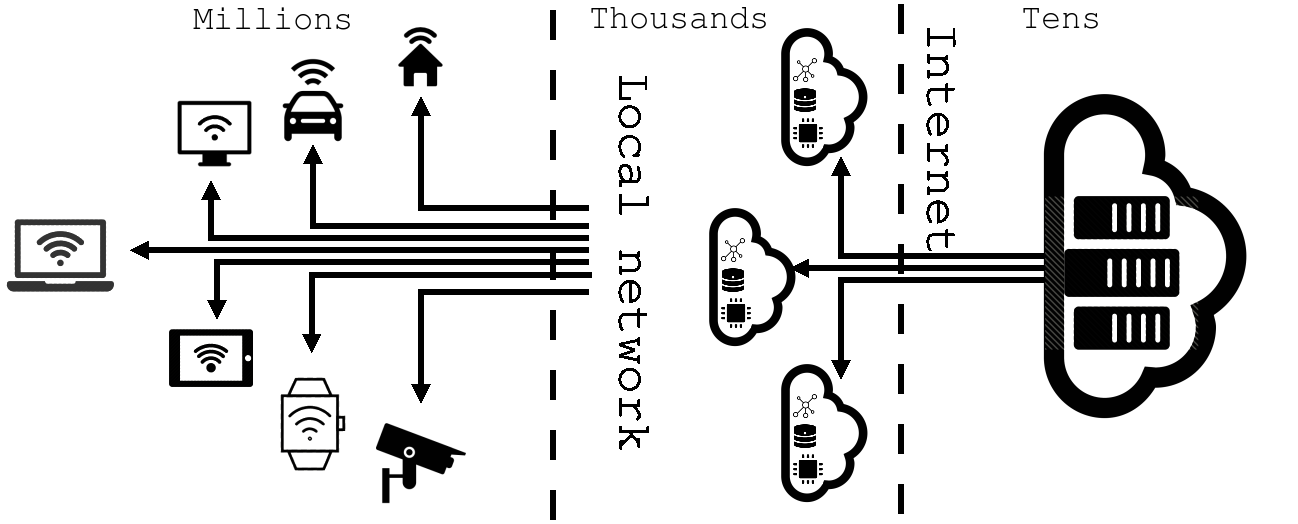
\includegraphics[width=0.9\linewidth]{figures/fog.png}
  
\end{figure}
\end{frame}
\end{withoutheadline}



\begin{withoutheadline}
\begin{frame}{The Fog}

\begin{block}{A Platform For The Fog}
    \begin{itemize}
    \item Fog computing is relatively new.
    \item<2-> The absence of a platform that assist fog architecture.
    \item<3-> A fog cluster can be built on top of cloud's platform like Kubernetes, Docker swarm, Mesos, Openstack.
    \item<4-> cloud's platform lack some complementary features that will full-fill the definition of fog. 
    \end{itemize}
\end{block} 
\end{frame}
\end{withoutheadline}



\subsection{PhD Objectives}

\begin{withoutheadline}
\begin{frame}{PhD Objectives}
\begin{block}{One broad Objective }
    \begin{itemize}
    \item Creating the optimized infrastructure control for fog computing architecture.
    \item<2-> This main objective will be achieved through 3 partial improvements:
    	\begin{itemize}
    		\item Taking the location and latency into account when assigning users to containers.
    		\item Changing the Kubernetes deployment controller, to allocate the containers in an optimized manner.
    		\item Decentralizing the infrastructure control of Kubernetes. 
    	\end{itemize}
    \end{itemize}
\end{block}
\end{frame}
\end{withoutheadline}

\section{Related Work}

\begin{withoutheadline}
\begin{frame}{Related Work }

\begin{block}{}
    \begin{itemize}
    \item Each objective has it's own set of related work. 
    \item For the broad objective, PiCasso is a new platform created for fog.
    \item For the Kubernetes service, Xie et al changing the services implementation by using IPVS instead of Iptables.
    \item For the platform decentralization, The Discovery initiative trying the same with openstack.
    
    \end{itemize}
\end{block}
\end{frame}
\end{withoutheadline}
